\section{Moti Laterali}

L'obiettivo del controllo dei moti laterali è quello di regolare il coefficiente di smorzamento e la frequenza naturale del sistema, così da garantire una risposta dinamica più desiderabile.

Studi condotti in ambito aeronautico \cite{franklin_feedback_control} hanno mostrato che i piloti tendono a preferire velivoli con coefficiente di smorzamento $\zeta > 0.5$ e frequenza naturale $\omega_n \approx 0.5$.

Poiché i requisiti sono espressi in termini di $\zeta$ e $\omega_n$, si preferisce utilizzare il luogo delle radici, in quanto consente di posizionare direttamente i poli del sistema in modo da soddisfare tali specifiche, risultando più appropriato rispetto alla sintesi di Bode.

\subsection{Controllore Proporzionale}

\subsubsection{Architettura}

\begin{figure}[H]
    \centering
    \begin{tikzpicture}
        \node[draw,
            circle,
            minimum size=0.5cm,
        ] (sum) at (0,0){};

        % Attuatore
        \node [draw,
            minimum width=2.4cm,
            minimum height=1.2cm,
            right=1cm of sum
        ]  (actuator) {$A(s)$};

        % System
        \node [draw,
            minimum width=2.4cm,
            minimum height=2.8cm,
            right=1.5cm of actuator,
            yshift=0.8cm
        ]  (system) {$Sistema$};

        % Controller
        \node [draw,
            minimum width=2.4cm,
            minimum height=1.2cm,
            below left= 1cm and -2.4cm of actuator
        ]  (controller) {$C(s) = k$};

        % Sensor block
        \node [draw,
            minimum width=2.4cm,
            minimum height=1.2cm,
            below right= 1cm and 1cm of actuator
        ]  (sensor) {$Giroscopio$};

        \draw[-stealth] (system.east) -- ++ (1.25,0)
        node[midway](output){}node[midway,above]{$r(t)$};

        \draw[stealth-] (system.150) -- ++ (-1.5,0)
        node[midway,above]{$\delta_a(t)$};

        \draw[-stealth] (sensor.west) -- ++ (-1,0);

        \draw[-stealth] (actuator.east) -- ++ (1.5,0)
        node[midway,above]{$\delta_r(t)$};

        \draw[-stealth] (sum.east) -- ++ (1,0);
        \draw[stealth-] (sum.west) -- ++ (-1.25,0)
        node[midway,above]{$\hat{r}(t)$};

        \draw[-stealth] (controller.west) -| (sum.south);

        \draw[-stealth] (output.center) |- (sensor.east);

        \node at ($(sum)+(-0.25,0.40)$) {$+$};
        \node at ($(sum)+(-0.25,-0.4)$) {$-$};
    \end{tikzpicture}
\end{figure}

Dove il blocco $A(s) = \frac{10}{s+10}$ è un modello dell'attuatore che è un componente a risposta più veloce rispetto al resto del sistema.
Presenta un unico polo in $-10$, il che implica tempi di salita e assestamento molto ridotti.

\subsubsection{Analisi del Parametro K}
Utilizzando il tool \texttt{Control System Designer}, si osserva che valori di $k > 0$ non sono adatti al controllo del sistema.
All'aumentare di $k$, infatti, i poli complessi coniugati associati al modo \textit{dutch roll} si spostano verso destra nel piano complesso.
In una fase iniziale ciò comporta una diminuzione del coefficiente di smorzamento $\zeta$; tuttavia, per valori di $k \gtrsim 0.1946$, i poli assumono parte reale positiva, portando all'instabilità del sistema.
\\[10pt]
Anche per valori di $k < 0$ si osserva come il controllore considerato non sia in grado di soddisfare i requisiti specificati dal problema.
Impostando tali vincoli all'interno del tool \texttt{Control System Designer}, si osserva che, per qualunque valore di $k$, i poli associati al moto di \textit{dutch roll} non rientrano mai nell'area bianca, indicativa delle posizioni nel piano compatibili con le specifiche di progetto.
\\[10pt]
Viene comunque determinato un valore del parametro $k$ che avvicina il più possibile al coefficiente di smorzamento richiesto, per fare ciò è stata utilizzata la funzionalità di \textit{optimization based tuning} fornita dal tool \texttt{Control System Designer}.

\begin{equation*}
    C_1(s) = -2.6981
\end{equation*}

\begin{figure}[H]
    \centering
    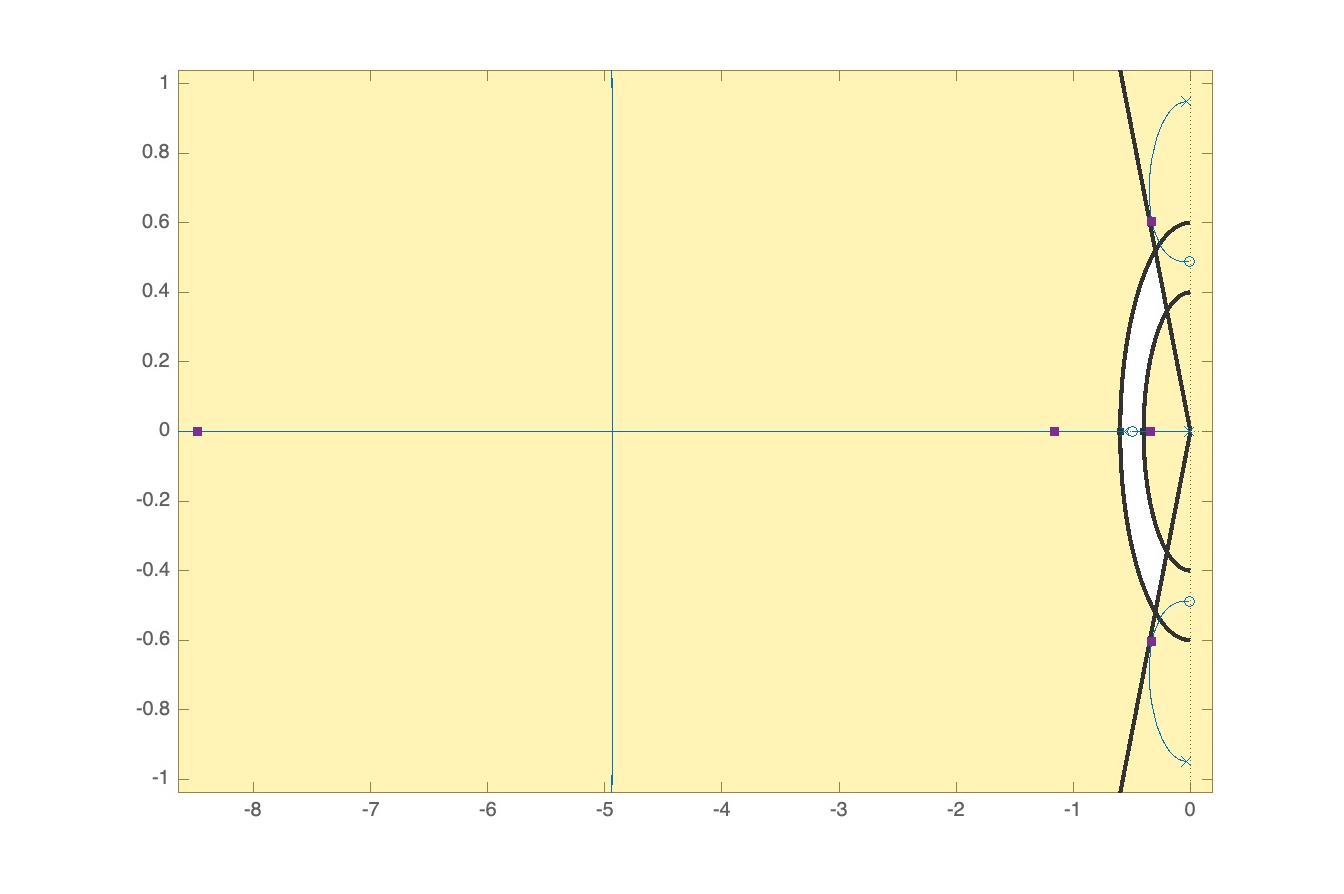
\includegraphics[width=0.6\linewidth]{Immagini/root_proportional_lateral.pdf}
    \caption{Luogo delle radici per $K < 0$ con segnate le radici per $K_1 = -2.6981$}
\end{figure}

\begin{figure}[H]
    \centering
    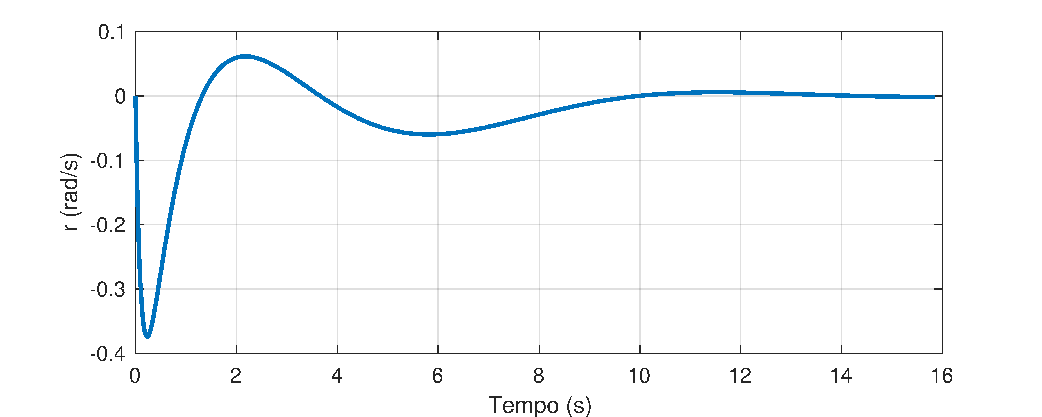
\includegraphics[width=0.7\linewidth]{Immagini/proportional_impulse_lateral.pdf}
    \caption{Risposta impulsiva del sistema con controllore proporzionale per $K_1 = -2.6981$}
\end{figure}

\subsubsection{Prestazioni}
Per il valore di $K_1$ ottenuto mediante ottimizzazione, si ricavano i seguenti parametri del sistema:
\begin{sitemize}
    \item coefficiente di smorzamento associato al modo \textit{dutch roll}: $\zeta_1 = 0.479$
    \item frequenza naturale associata al modo \textit{dutch roll}: $\omega_{n, 1} = 0.686\, rad/s$
    \item tempo di salita: $T_{s, 1} = 7.26 \, s$
    \item sovraelongazione percentuale: $S_{\%, 1} = 2.43\%$
    \item tempo di assestamento: $T_{a, 1} = 10.7 \, s$
\end{sitemize}

\begin{figure}[H]
    \centering
    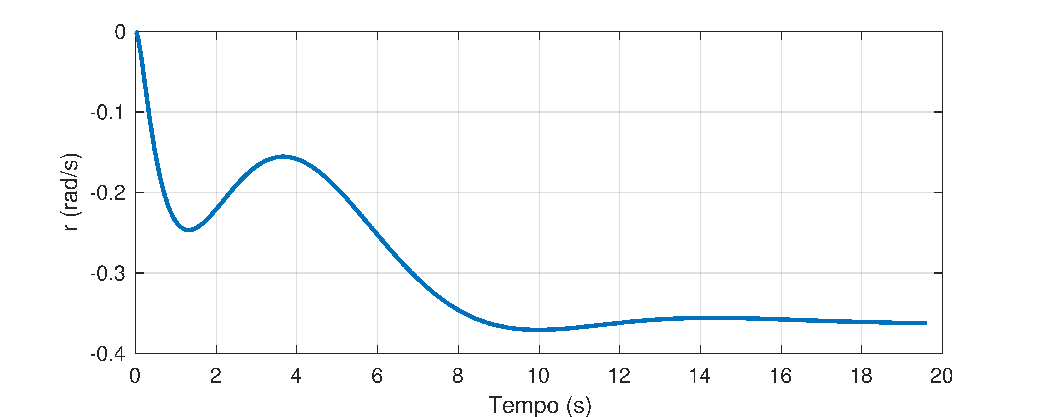
\includegraphics[width=0.7\linewidth]{Immagini/proportional_step_lateral.pdf}
    \caption{Risposta al gradino del sistema con controllore proporzionale per $K_1 = -2.6981$}
\end{figure}

Sebbene i requisiti specificati non risultino pienamente soddisfatti, i valori ottenuti si avvicinano sensibilmente alle specifiche, soprattutto se si considera la semplicità dell'architettura di controllo adottata.

\subsection{Controllore a Singolo Polo}

\subsubsection{Architettura}
L'architettura del sistema di controllo rimane sostanzialmente invariata; viene tuttavia sostituito il controllore proporzionale con un controllore a singolo polo, descritto dalla seguente funzione di trasferimento:
\begin{equation*}
    C(s) = \frac{K}{s + p_0}
\end{equation*}

\subsubsection{Analisi dei Parametri \texorpdfstring{$p_0$}{p0} e K}\label{subsubsec:analisi_parametri_controllore_polo_singolo}
La scelta della posizione del polo reale viene eseguita sperimentalmente:
\begin{sitemize}
    \item Per valori di $p_0$ nell'intervallo $[-3.045, 0]$, la presenza del polo fa sì che i poli associati al modo \textit{dutch roll} seguano un percorso che li allontana dall'asse reale e li avvicina a quello immaginario, peggiorando così le prestazioni del sistema.
    \item Per valori di $p_0 < -3.045$, l'effetto si inverte: il percorso dei poli del modo \textit{dutch roll} si avvicina all'asse reale e si allontana da quello immaginario, migliorando così le prestazioni del sistema. Il massimo effetto positivo si ottiene proprio per $p_0 = -3.045$.
\end{sitemize}

La scelta del parametro $K$ avviene similmente a quanto fatto precedentemente per il controllore proporzionale determinando così il valore di $K_2 = -9.202$

\begin{equation*}
    C_2(s) = -\frac{9.202}{s + 3.045} = -\frac{3.022}{1 + 0.3268s}
\end{equation*}

\begin{figure}[H]
    \centering
    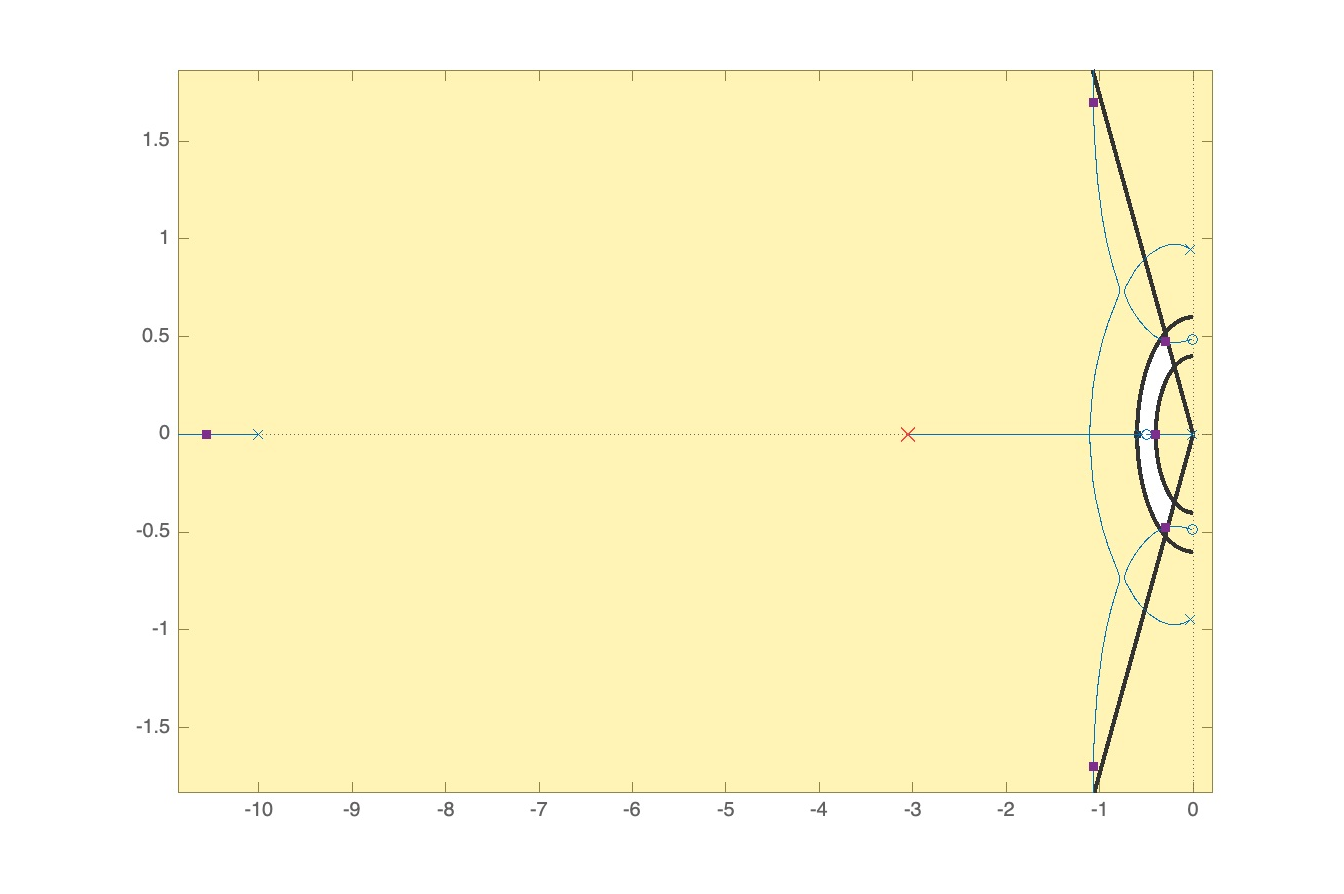
\includegraphics[width=0.6\linewidth]{Immagini/root_pole_lateral.pdf}
    \caption{Luogo delle radici per $K < 0$ con segnate le radici per $K_2 = -9.202$ e $p_0 = -3.045$}
\end{figure}

\begin{figure}[H]
    \centering
    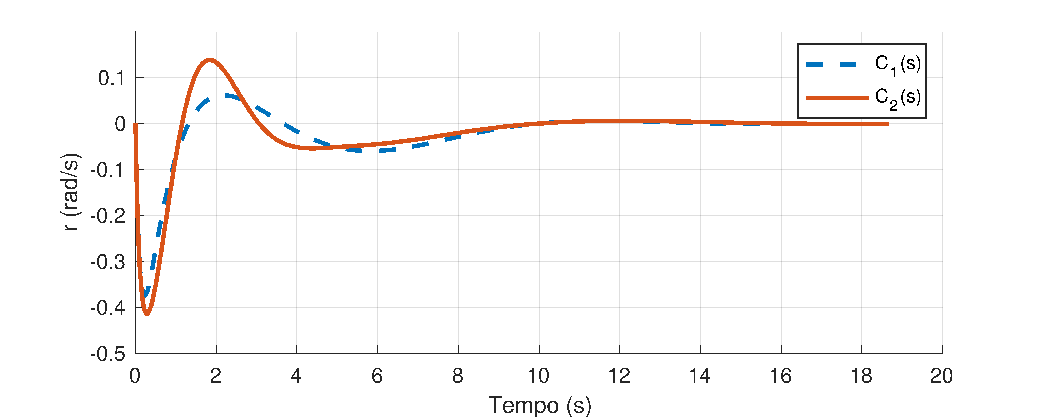
\includegraphics[width=0.7\linewidth]{Immagini/pole_impulse_lateral.pdf}
    \caption{Risposta impulsiva del sistema con controllore a singolo polo per $K_2 = -9.202$ e $p_0 = -3.045$}
\end{figure}

\subsubsection{Prestazioni}
Per i valori di $p_0$ e $K_2$ si ricavano i seguenti parametri del sistema:
\begin{sitemize}
    \item coefficiente di smorzamento associato al modo \textit{dutch roll}: $\zeta_2 = 0.527$
    \item frequenza naturale associata al modo \textit{dutch roll}: $\omega_{n, 2} = 0.559 \, rad/s$
    \item tempo di salita: $T_{s, 2} = 6.71 \, s$
    \item sovraelongazione percentuale: $S_{\%, 2} = 5.52\%$
    \item tempo di assestamento: $T_{a, 2} = 12.7 \, s$
\end{sitemize}

\begin{figure}[H]
    \centering
    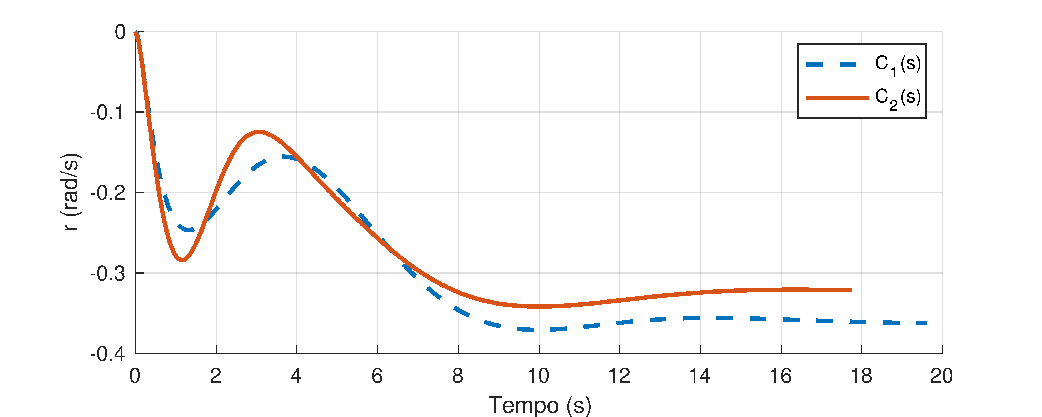
\includegraphics[width=0.7\linewidth]{Immagini/pole_step_lateral.pdf}
    \caption{Risposta dell'angolo di rollio al gradino del sistema con controllore a singolo polo per $K_2 = -9.202$ e $p_0 = -3.045$}
\end{figure}

In questo caso, il controllore a singolo polo consente di soddisfare i requisiti specificati dal problema.

\subsection{Effetti Negativi della Retroazione}

Come descritto in \cite{mathworks_yaw_damper}, i controllori precedentemente descritti si rivelano problematici nel momento in cui il pilota cerca di imporre un angolo di rollio costante al velivolo. In tali condizioni, infatti, il controllore genera dei comandi che tendono ad annullare l'azione del pilota.

La funzione di trasferimento è stata quindi sovrastabilizzata, attenuando eccessivamente il modo \textit{spiral}, al quale i piloti sono abituati e che si aspettano.

\begin{figure}[H]
    \centering
    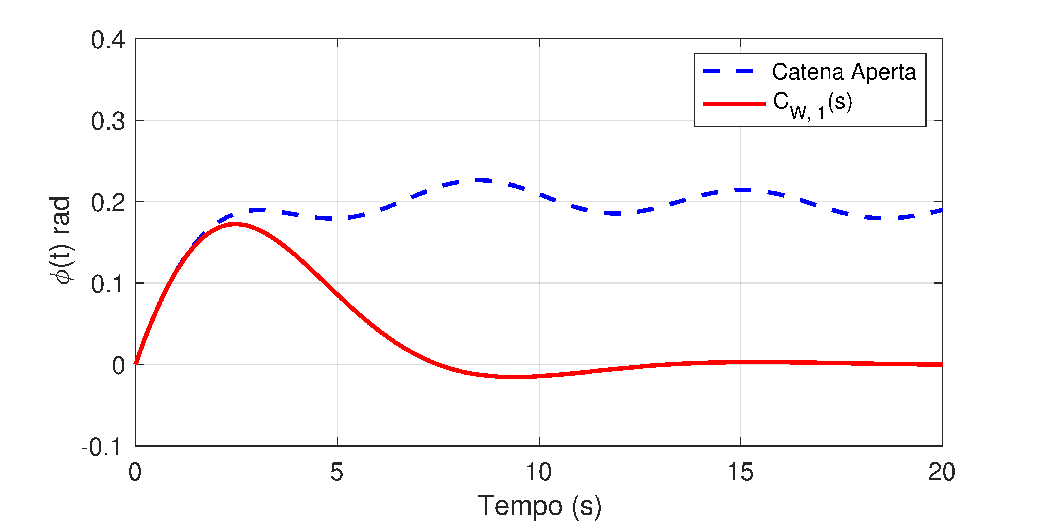
\includegraphics[width=0.7\linewidth]{Immagini/effetto_negativo_retroazione.pdf}
    \caption{Risposta del sistema ad un impulso agli alettoni}
\end{figure}

I piloti sono abituati a questo comportamento del velivolo. Per reintrodurlo nel sistema controllato, si introduce nella retroazione un filtro passa-alto, noto come \textit{washout filter}, il cui scopo è attenuare la risposta del controllore a segnali costanti o a bassa frequenza.

\subsubsection{Architettura}

\begin{figure}[H]
    \centering
    \begin{tikzpicture}
        \node[draw,
            circle,
            minimum size=0.5cm,
        ] (sum) at (0,0){};

        % Attuatore
        \node [draw,
            minimum width=2.4cm,
            minimum height=1.2cm,
            right=1cm of sum
        ]  (actuator) {$A(s)$};

        % System
        \node [draw,
            minimum width=2.4cm,
            minimum height=2.8cm,
            right=1.5cm of actuator,
            yshift=0.8cm
        ]  (system) {$Sistema$};

        % Sensor block
        \node [draw,
            minimum width=2.4cm,
            minimum height=1.2cm,
            below right= 1cm and 5.2cm of sum
        ]  (sensor) {$Giroscopio$};

        % washout block
        \node [draw,
            minimum width=1.6cm,
            minimum height=1.2cm,
            below right= 1cm and 2.8 cm of sum
        ]  (washout) {$W(s)$};

        % Controller
        \node [draw,
            minimum width=1.6cm,
            minimum height=1.2cm,
            below right=1cm and 0.4 cm of sum
        ]  (controller) {$C(s)$};

        \draw[-stealth] (system.east) -- ++ (1.25,0)
        node[midway](output){}node[midway,above]{$r(t)$};

        \draw[stealth-] (system.150) -- ++ (-1.5,0)
        node[midway,above]{$\delta_a(t)$};

        \draw[-stealth] (washout.west) -- ++ (-0.8,0);

        \draw[-stealth] (actuator.east) -- ++ (1.5,0)
        node[midway,above]{$\delta_r(t)$};

        \draw[-stealth] (sum.east) -- ++ (1,0);
        \draw[stealth-] (sum.west) -- ++ (-1.25,0)
        node[midway,above]{$\hat{r}(t)$};

        \draw[-stealth] (sensor.west) -- ++ (-0.8, 0);

        \draw[-stealth] (controller.west) -| (sum.south);

        \draw[-stealth] (output.center) |- (sensor.east);

        \node at ($(sum)+(-0.25,0.40)$) {$+$};
        \node at ($(sum)+(-0.25,-0.4)$) {$-$};
    \end{tikzpicture}
\end{figure}

Dove il controllore è a singolo polo e il filtro passa-alto $W(s)$ è definito come:
\begin{equation*}
    W(s) = \frac{s}{s + \frac{1}{\tau}}
\end{equation*}

Il parametro $\tau$ determina la frequenza di taglio del filtro e può essere regolato in base ai requisiti del sistema.

\subsubsection{Analisi del Parametro \texorpdfstring{$\tau$}{tau}}

Vengono ora analizzate le prestazioni del sistema al variare del parametro $\tau$, i controllori utilizzati per questa analisi sono stati progettati seguendo il metodo precedentemente descritto nella sezione \ref{subsubsec:analisi_parametri_controllore_polo_singolo}.
\renewcommand{\arraystretch}{2}
\begin{table}[H]
    \centering
    \begin{tabularx}{\textwidth}{@{}l *7{>{\centering\arraybackslash}X}@{}}
        \toprule
        \textbf{Controllore}                     & {$\tau$} & {$\zeta$} & {$\omega_n$ [rad/s]} & {$t_r$ [s]} & {$t_a$ [s]} \\
        \midrule
        $C_{W, 1}(s) = -\dfrac{1.635}{1+ 0.59s}$ & 3        & 0.5       & 0.839                & 470         & 835         \\
        $C_{W, 2}(s) = -\dfrac{2.106}{1+ 0.47s}$ & 5        & 0.503     & 0.689                & 663         & 1180        \\
        $C_{W, 3}(s) = -\dfrac{2.614}{1+ 0.39s}$ & 10       & 0.5       & 0.608                & 1249        & 2128        \\
        \bottomrule
    \end{tabularx}
    \label{tab:compensatori}
\end{table}

Si osserva che valori più bassi di $\tau$ tendono a favorire la risposta del sistema agli ingressi costanti, mentre valori più elevati migliorano la stabilità del sistema.

Questo accade perché, all'aumentare di $\tau$ il polo associato al filtro di \textit{washout} si avvicina all'origine del piano complesso, consentendo di ottenere valori più favorevoli per $\zeta$ e $\omega_n$, a discapito però dei tempi di risposta, che risultano peggiorati.

Dal punto di vista fisico, un incremento di $\tau$ comporta una riduzione della frequenza di taglio del filtro passa-alto, estendendo così l'intervallo di frequenze su cui il controllore esercita un'influenza significativa.

\begin{figure}[H]
    \centering
    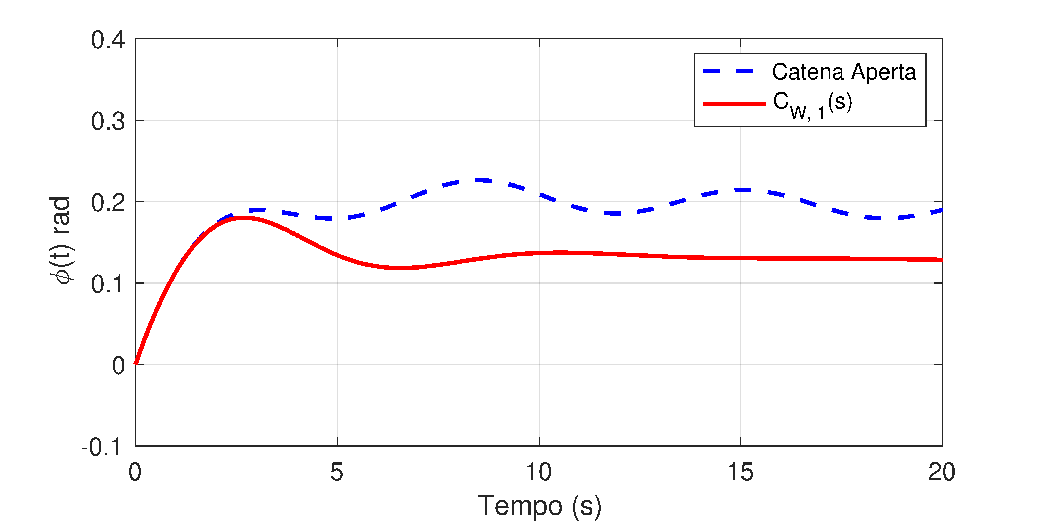
\includegraphics[width=0.7\linewidth]{Immagini/washout_altettone.pdf}
    \caption{Risposta del sistema ad un impulso agli alettoni con filtro di \textit{washout} nel caso $\tau = 3$}
\end{figure}


\begin{figure}[H]
    \centering
    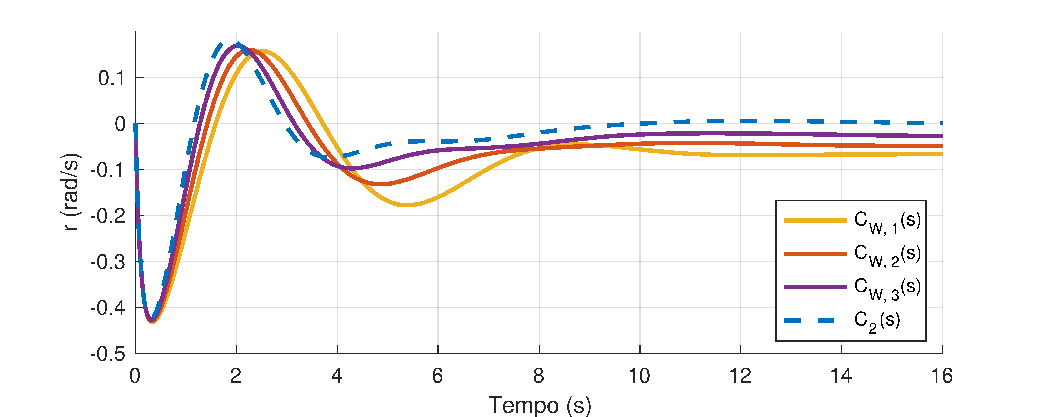
\includegraphics[width=0.7\linewidth]{Immagini/washout_impulse.pdf}
    \caption{Risposta impulsiva dei controllori con filtro di \textit{washout}}
\end{figure}

\begin{figure}[H]
    \centering
    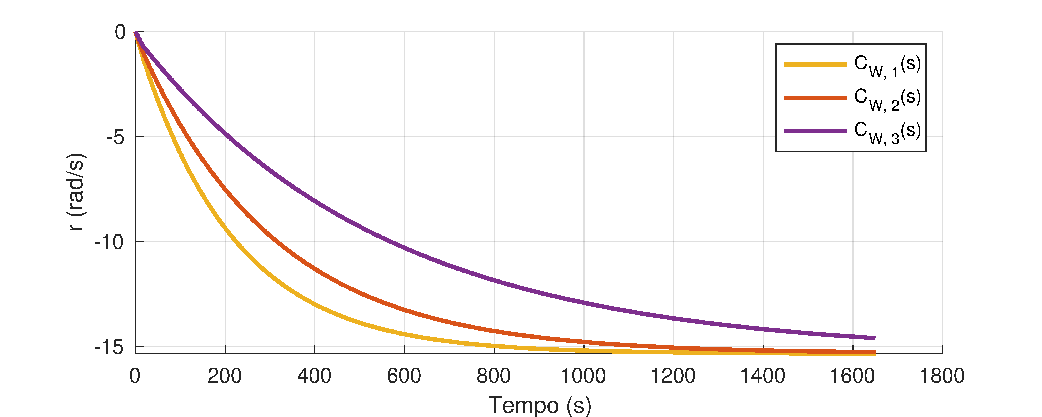
\includegraphics[width=0.7\linewidth]{Immagini/washout_step.pdf}
    \caption{Risposta al gradino dei controllori con filtro di \textit{washout}}
\end{figure}

\begin{note}
    Si nota che il filtro di \textit{washout} può essere integrato nel controllore, per ottenere tale controllore è sufficiente moltiplicare le funzioni di trasferimento del controllore e del filtro passa-alto.
\end{note}

\subsection{Sintesi con Strategia di Controllo Ottimo}
Si osserva che le prestazioni del sistema di controllo possono essere migliorate utilizzando un controllore \textit{full-state feedback}, questa strategia viene descritta in dettaglio in \cite{franklin_feedback_control}.

Tuttavia, come sottolineato nel testo, tale strategia comporta un aumento della complessità del sistema non giustificato dal miglioramento marginale delle prestazioni. Per questa ragione, il suo impiego risulta poco diffuso nella pratica.
